\section{بخش سوم: بخش‌بندی با روش برش نرمال‌شده (\lr{Normalized Cut})}

\begin{stepbox}
\field{استفاده از تئوری گراف در پردازش تصویر}{
در روش \lr{Normalized Cut} که یکی از خواسته‌های اصلی این بخش از تمرین است[cite: 1]، تصویر به عنوان یک گراف مدل‌سازی می‌شود که در آن مجموعه‌ای از پیکسل‌ها نقش گره‌ها (\lr{Nodes}) را ایفا می‌کنند و لبه‌های گراف نشان‌دهنده‌ی میزان شباهت بین آن‌هاست. 

به دلیل حجم بسیار بالای محاسبات گراف برای تک‌تک پیکسل‌های یک تصویر با وضوح بالا، ابتدا از الگوریتم \lr{SLIC} برای تقسیم تصویر به قطعاتی به نام «سوپرپیکسل» استفاده می‌شود. سپس گراف مجاورت نواحی (\lr{RAG}) بر روی این سوپرپیکسل‌ها تشکیل شده و الگوریتم، گراف را از ضعیف‌ترین پیوندها برش می‌دهد.
}
\end{stepbox}

\begin{codebox}[پیاده‌سازی \lr{Normalized Cut} با کتابخانه‌ی \lr{skimage}]
\begin{lstlisting}[language=Python]
import time
from skimage import segmentation, color, graph

start_time = time.time()
labels1 = segmentation.slic(image_rgb, compactness=30, n_segments=200, start_label=1)

rag = graph.rag_mean_color(image_rgb, labels1, mode='similarity')

labels2 = graph.cut_normalized(labels1, rag)
out_ncut = color.label2rgb(labels2, image_rgb, kind='avg', bg_label=0)

print(f"Time: {time.time() - start_time:.2f}s")
\end{lstlisting}
\end{codebox}
\newpage
\begin{stepbox}
\field{تحلیل و بررسی نتایج بر روی تصاویر مختلف}{
عملکرد الگوریتم \lr{Normalized Cut} به شدت به ساختار محتوایی تصویر و پارامترهای تعداد گره‌ها ($n$) و فشردگی ($c$) بستگی دارد. بررسی نتایج روی سه تصویر با ویژگی‌های متفاوت، نکات زیر را نشان می‌دهد:

\begin{itemize}
    \item \textbf{تصویر اسب (سوژه بزرگ با رنگ مشابه پس‌زمینه):} در این تصویر، استفاده از تعداد گره‌های کمتر ($n=100$) بهترین نتیجه را برای جداسازی اسب به همراه داشت. با افزایش تعداد سوپرپیکسل‌ها به $400$، به دلیل شباهت رنگی زیاد بین موهای اسب و گرد و خاک پس‌زمینه، گراف به شدت پیچیده شده و الگوریتم دچار خطای ادغام (\lr{Under-segmentation} در سوژه اصلی) گردید که منجر به تولید یک لکه‌ی خاکستری نامفهوم شد.
    
    \item \textbf{تصویر ماهی‌ها (جزئیات ریز و پراکنده با رنگ‌های متضاد):} برخلاف اسب، در این تصویر به دلیل وجود ماهی‌های کوچک و مرجان‌ها، گره‌های کم ($n=100$) باعث از بین رفتن کامل ماهی‌های کوچکتر و ادغام آن‌ها با آب دریا شد. با افزایش پارامترها به $c=30, n=200$، تعادل خوبی برقرار شد و ماهی‌های اصلی به خوبی از آب تفکیک شدند. در حالت $n=400$، اگرچه جزئیات ریزتری استخراج شد، اما پس‌زمینه (آب دریا) دچار بیش‌بخش‌بندی (\lr{Over-segmentation}) و تکه‌تکه شدن گردید.
    
    \item \textbf{تصویر پلنگ سیاه (سوژه تیره و یکدست روی بافت شلوغ):} بدن پلنگ سیاه دارای رنگی پیوسته و تیره است. در حالت $c=30, n=200$ الگوریتم توانست به خوبی مرز بین بافت سبز چمن‌ها و تیرگی بدن پلنگ را تشخیص دهد. اما با افزایش حساسیت و تعداد گره‌ها به $400$، بازتاب‌های نوری روی موهای پلنگ باعث شد تا بدن یکپارچه‌ی حیوان دچار تکه‌تکه شدن شود و یکپارچگی سوژه از دست برود.
\end{itemize}
}
\end{stepbox}

\begin{figure}[h!]
    \centering
    % مسیر تصویر را در صورت نیاز با توجه به نام فایل خود اصلاح کنید
    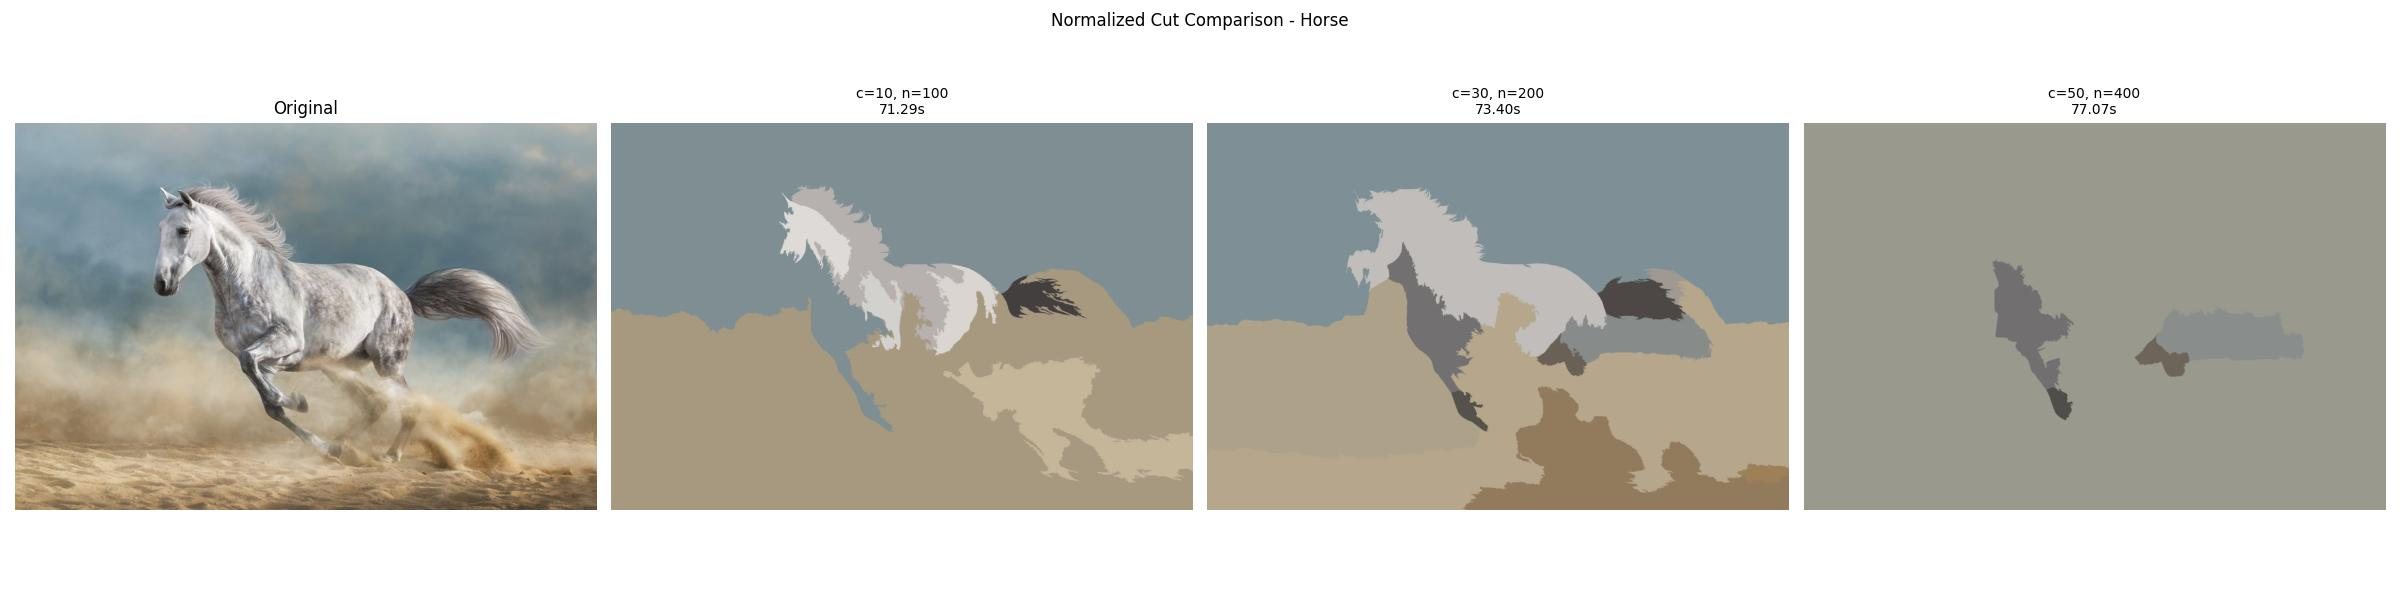
\includegraphics[width=\textwidth]{./images/Part_3/Horse_NCut_Comparison.jpg}
    \caption{تأثیر پارامترهای الگوریتم \lr{Normalized Cut} روی تصویر اسب؛ افزایش گره‌ها منجر به افت شدید کیفیت بخش‌بندی شده است.}
    \label{fig:ncut_horse}
\end{figure}

\begin{figure}[h!]
    \centering
    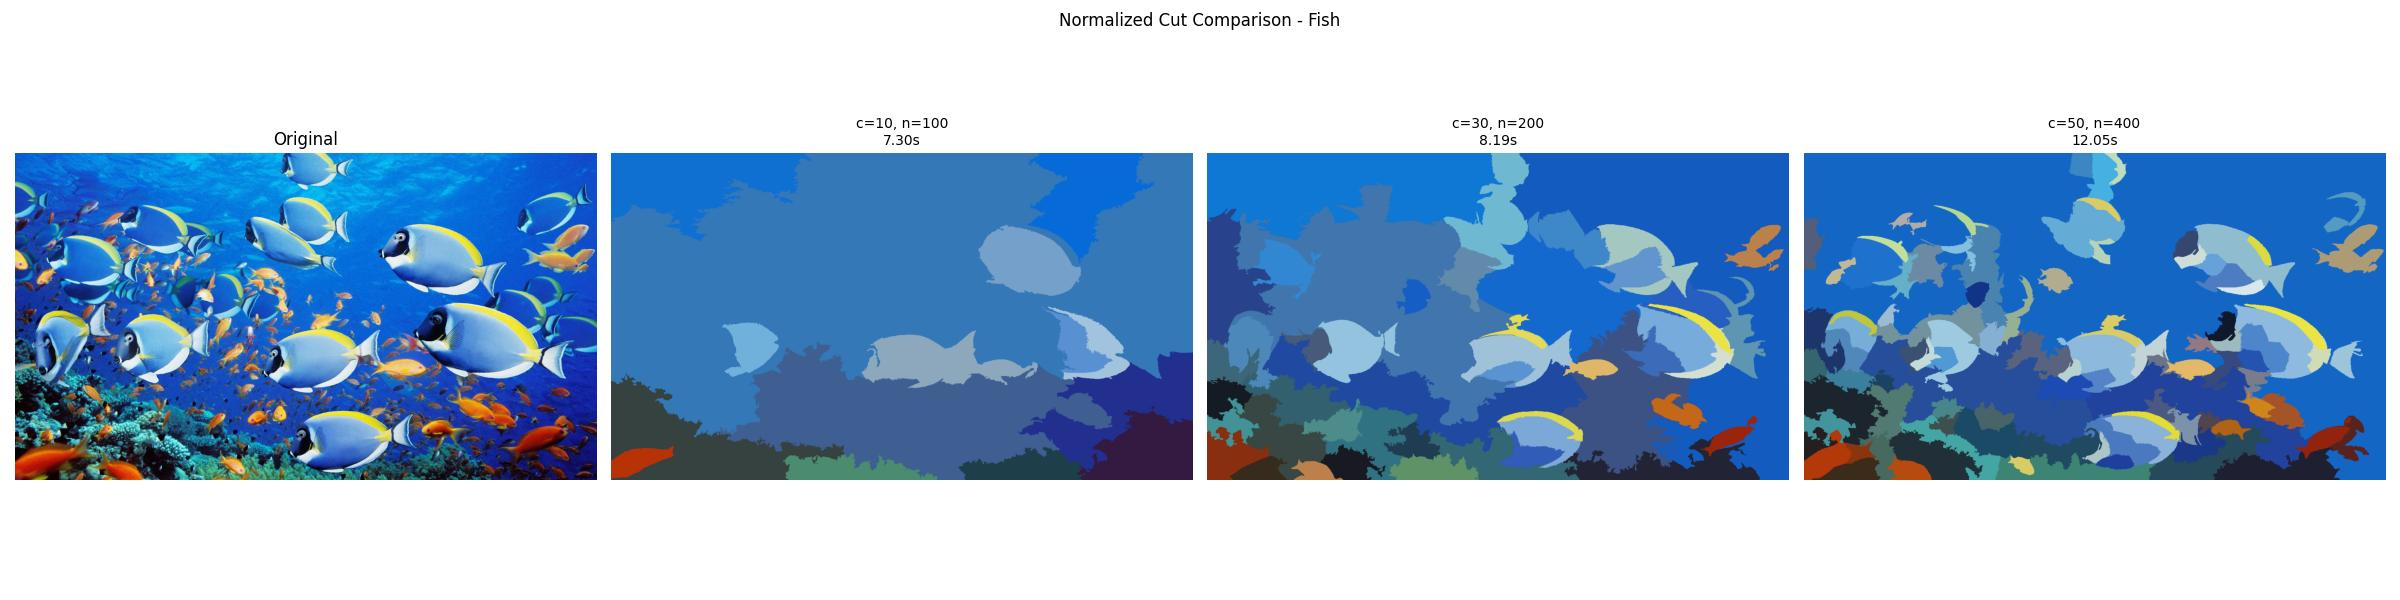
\includegraphics[width=\textwidth]{./images/Part_3/Fish_NCut_Comparison.jpg}
    \caption{تأثیر پارامترهای الگوریتم \lr{Normalized Cut} روی تصویر ماهی؛ برای استخراج جزئیات پراکنده، نیاز به تعداد گره‌های بالاتری است.}
    \label{fig:ncut_fish}
\end{figure}

\begin{figure}[h!]
    \centering
    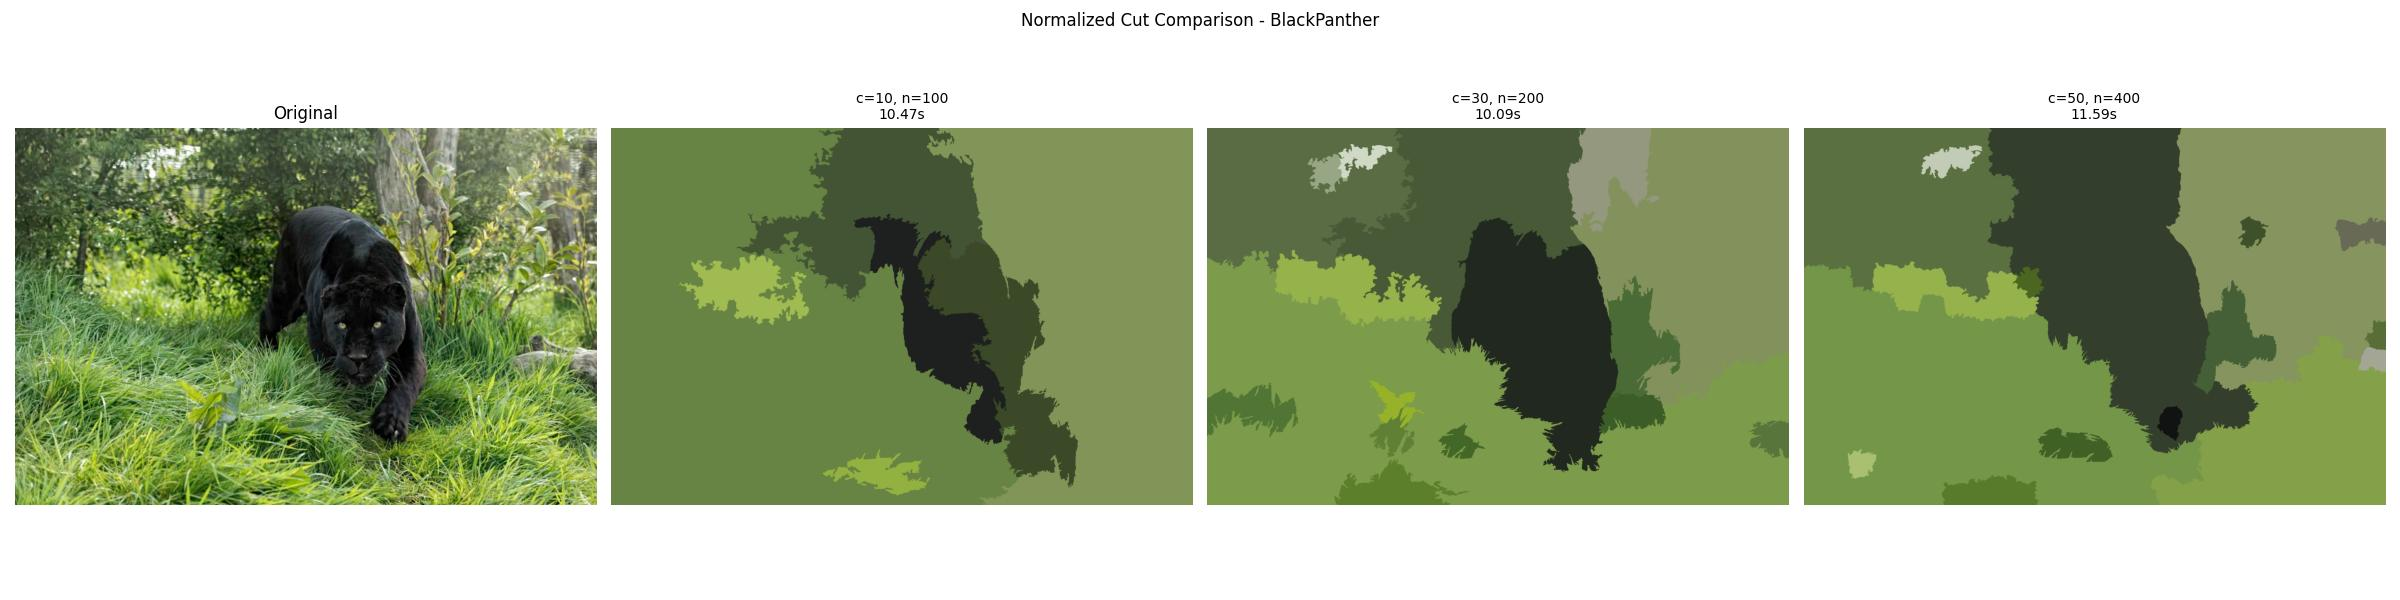
\includegraphics[width=\textwidth]{./images/Part_3/BlackPanther_NCut_Comparison.jpg}
    \caption{تأثیر پارامترهای الگوریتم \lr{Normalized Cut} روی تصویر پلنگ؛ حالت $n=200$ بهترین تعادل را برای حفظ یکپارچگی سوژه ایجاد کرده است.}
    \label{fig:ncut_panther}
\end{figure}

\begin{warnbox}[حساسیت به پیچیدگی گراف]
بررسی جامع خروجی‌ها نشان می‌دهد که در تئوری گراف، بزرگ کردن پارامترها لزوماً خروجی بهتری تولید نمی‌کند. برای سوژه‌های بزرگ و یکدست، گراف‌های ساده‌تر (سوپرپیکسل‌های کمتر) و برای تصاویر پرجزئیات، گراف‌های متراکم‌تر مناسب هستند. تنظیم این پارامتر کاملاً به ماهیت بصری عکس وابسته است.
\end{warnbox}